\documentclass[parskip=full]{scrartcl}

\usepackage{amsmath}
\usepackage{hyperref}
\usepackage{graphicx}
\graphicspath {{images/}}
\hypersetup{
    colorlinks=true,
    citecolor=blue
}

\renewcommand\thesubsection{\thesection.\alph{subsection}}


\begin{document}


\title{CS698 - Assignment 3}
\subtitle{Winter 2017}
\author{
    Vineet John\\
    \texttt{v2john@uwaterloo.ca}
}
\date{\today}
\maketitle


\section{Gaussian Kernel Derivation} % (fold)
\label{sec:gaussian_kernel_derivation}



% section gaussian_kernel_derivation (end)


\section{Perceptron Learning Algorithm - Dual Formulation} % (fold)
\label{sec:perceptron_learning_algorithm_dual_formulation}



% section perceptron_learning_algorithm_dual_formulation (end)


\section{Non-linear Regression Techniques} % (fold)
\label{sec:non_linear_regression_techniques}

    \subsection{Regularized Generalized Linear Regression} % (fold)
    \label{sub:regularized_generalized_linear_regression}
    
        Figure \ref{fig:rglg_err_v_deg} shows how the model error varies with respect to the maximum degree of basis functions. The best performing basis function in terms of error minimization is the one with degree 4.

        \begin{figure}[ht]
            \centering
            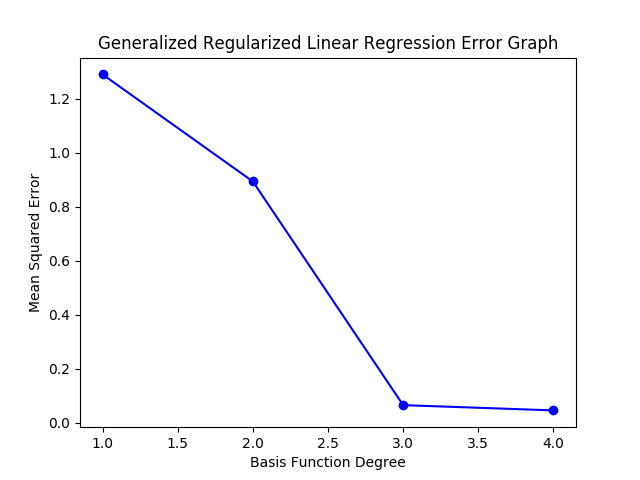
\includegraphics[width=0.6\textwidth]{3a_degree_vs_error.png}
            \caption{Regularized Generalized Linear Regression - Error vs Basis function degree}
            \label{fig:rglg_err_v_deg}
        \end{figure}

        Similarly, Figure \ref{fig:rglg_time_v_deg} shows the variation of time required for the computation as a function of the maximum basis function degree. The experiments might not be very indicative of the complexity increase, due to the low amount of time the computation actually takes, but the computation seems to be increasing monotonically for increased maximum degree of basis functions. This could be attributed to the increase of the size of the weights that need to be computed, because each `n' degree basis function is a subset of any `m' degree basis function $\forall m > n$

        \begin{figure}[ht]
            \centering
            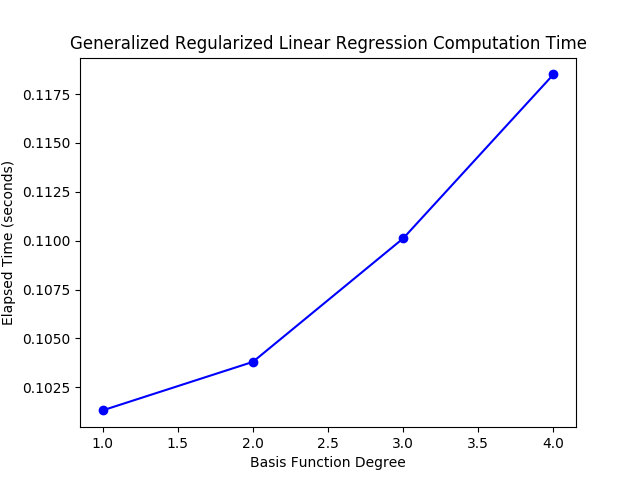
\includegraphics[width=0.6\textwidth]{3a_degree_vs_time.png}
            \caption{Regularized Generalized Linear Regression - Time vs Basis function degree}
            \label{fig:rglg_time_v_deg}
        \end{figure}

        The code for Regularized Generalized Linear Regression is present in the directory `regularized-generalized-linear-regression' of the code archive submitted.

    % subsection regularized_generalized_linear_regression (end)

    \subsection{Bayesian Generalized Linear Regression} % (fold)
    \label{sub:bayesian_generalized_linear_regression}
    
        \begin{figure}[ht]
            \centering
            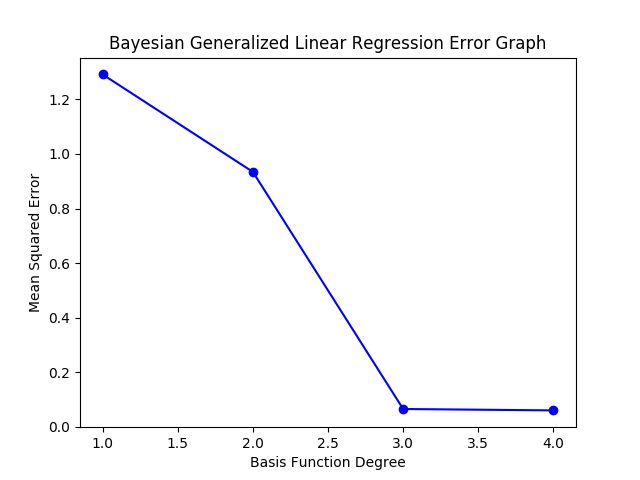
\includegraphics[width=0.6\textwidth]{3b_degree_vs_error.png}
            \caption{Bayesian Generalized Linear Regression - Error vs Basis function degree}
            \label{fig:bglg_err_v_deg}
        \end{figure}

        \begin{figure}[ht]
            \centering
            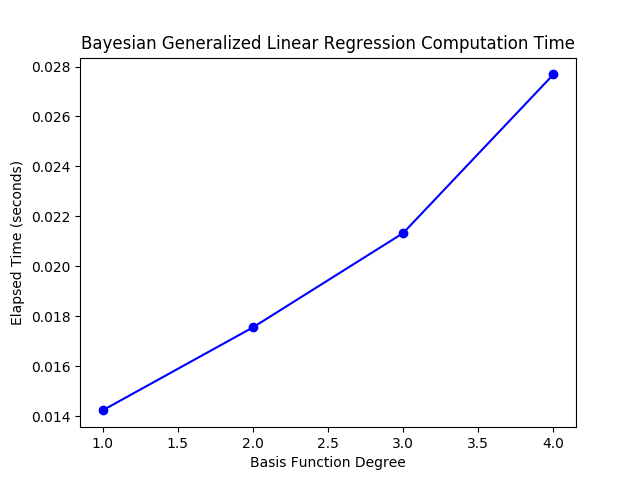
\includegraphics[width=0.6\textwidth]{3b_degree_vs_time.png}
            \caption{Bayesian Generalized Linear Regression - Time vs Basis function degree}
            \label{fig:bglg_time_v_deg}
        \end{figure}
    
    % subsection bayesian_generalized_linear_regression (end)

    \section{Gaussian Process Regression} % (fold)
    \label{sec:gaussian_process_regression}
    
    % section gaussian_process_regression (end)

% section non_linear_regression_techniques (end)


\end{document}
